\documentclass{standalone}
\usepackage{tikz}
\usetikzlibrary{patterns, positioning}
\usepackage[sfdefault]{ClearSans} %% option 'sfdefault' activates Clear Sans as the default text font
\usepackage[T1]{fontenc}

\begin{document}
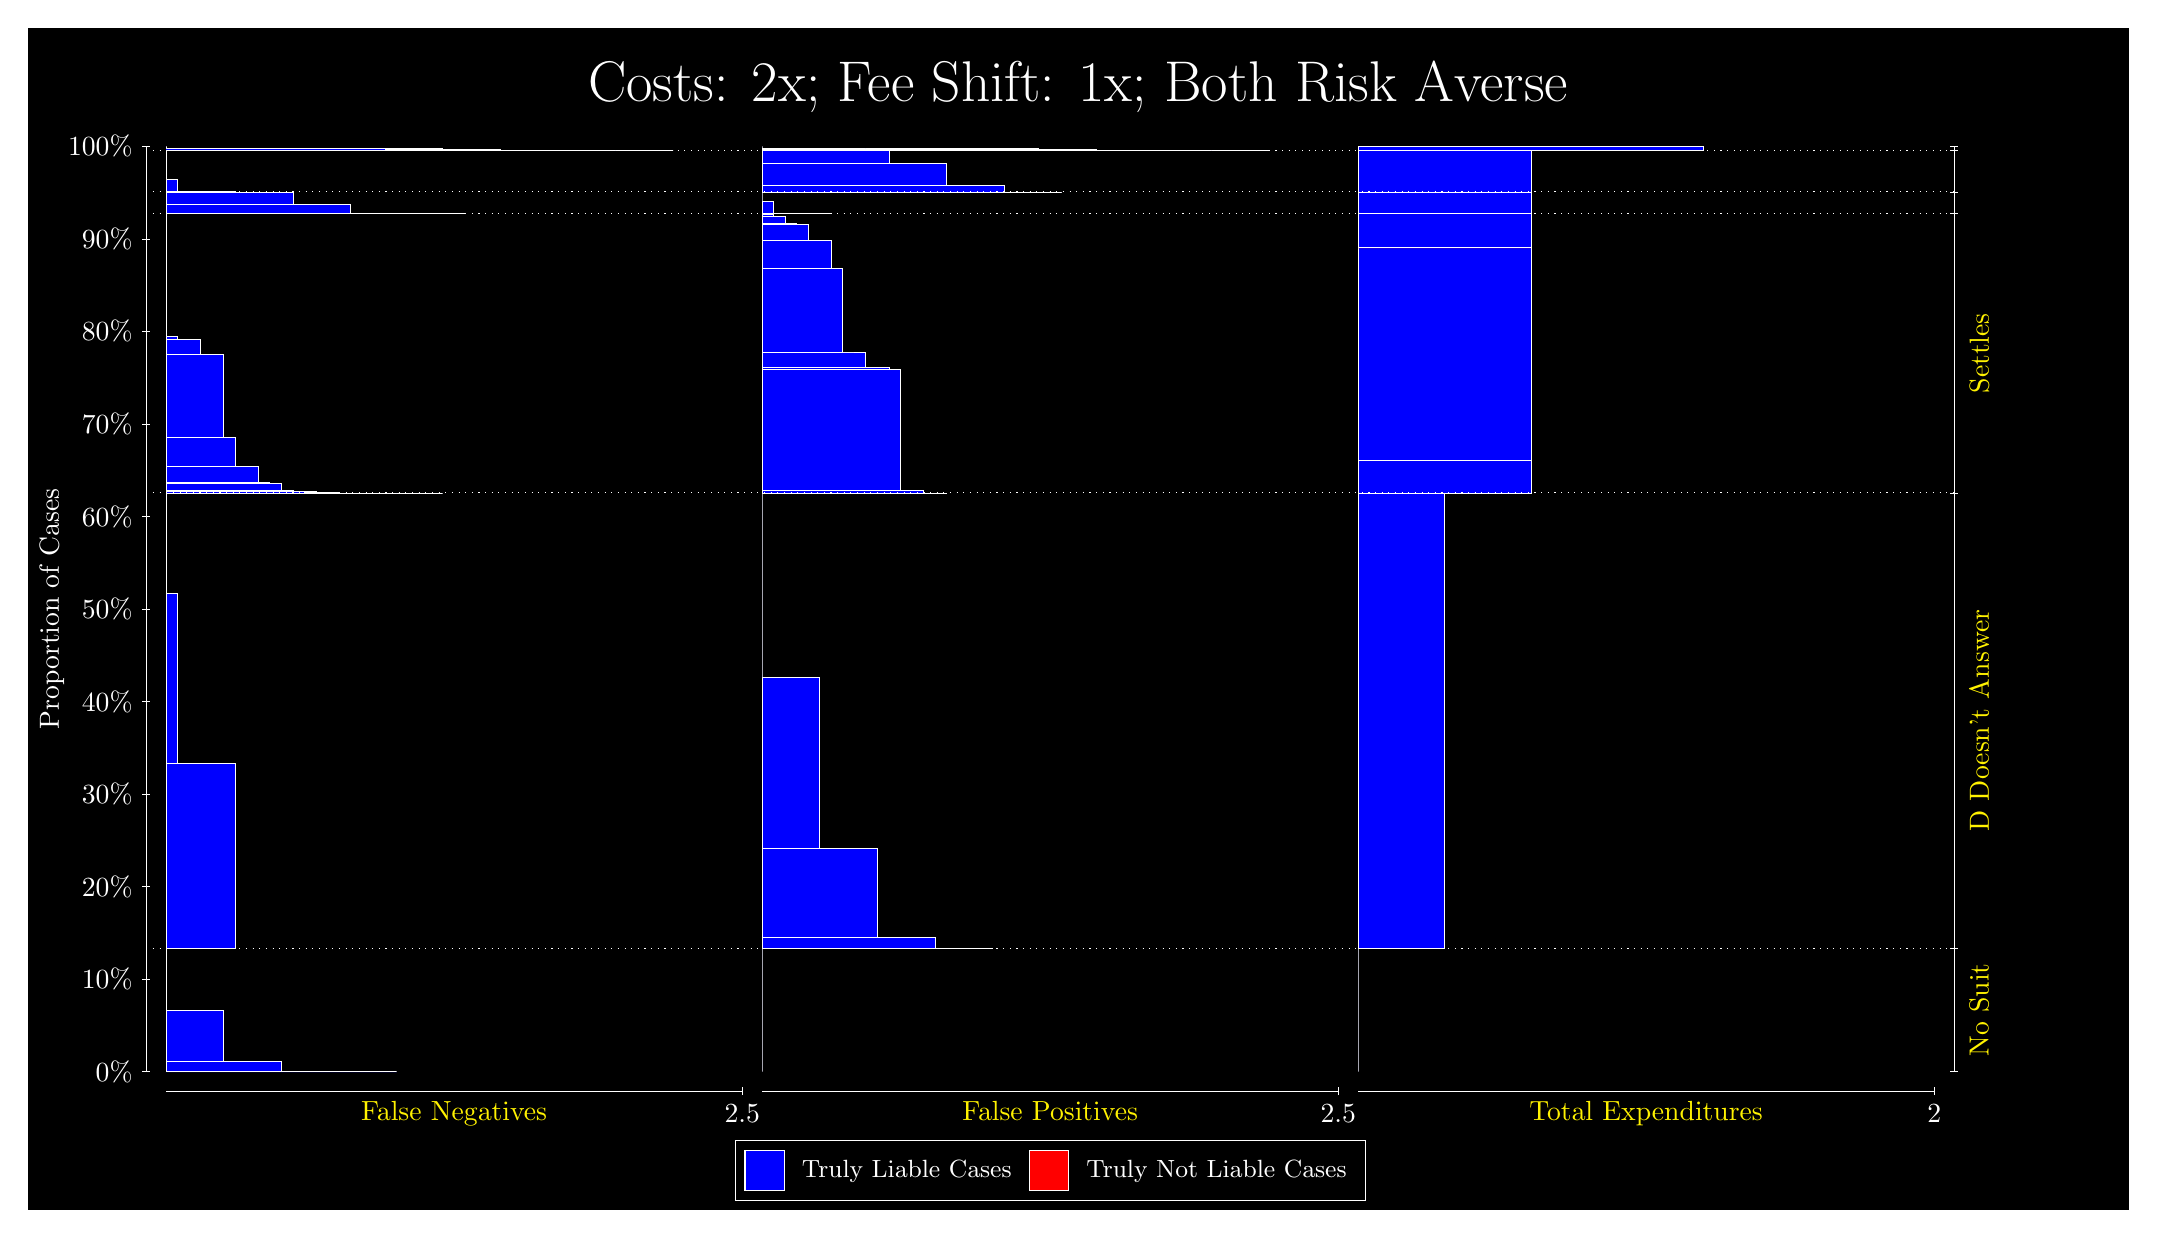
\begin{tikzpicture}
\draw[fill=black] (0,0) rectangle (26.667,15);
\draw[text=white] (0,13.5) rectangle (26.667,15) node[midway] {\huge Costs: 2x; Fee Shift: 1x; Both Risk Averse};
\draw[white, very thin] (1.5,1.75) -- (1.5,13.5);
\node[rotate=90, text=white, anchor=center] at (0.3, 7.625) {Proportion of Cases};
\draw[white, very thin] (1.45,1.75) -- (1.55,1.75);
\node[text=white, anchor=east] at (1.45, 1.75) {0\%};
\draw[white, very thin] (1.45,2.925) -- (1.55,2.925);
\node[text=white, anchor=east] at (1.45, 2.925) {10\%};
\draw[white, very thin] (1.45,4.1) -- (1.55,4.1);
\node[text=white, anchor=east] at (1.45, 4.1) {20\%};
\draw[white, very thin] (1.45,5.275) -- (1.55,5.275);
\node[text=white, anchor=east] at (1.45, 5.275) {30\%};
\draw[white, very thin] (1.45,6.45) -- (1.55,6.45);
\node[text=white, anchor=east] at (1.45, 6.45) {40\%};
\draw[white, very thin] (1.45,7.625) -- (1.55,7.625);
\node[text=white, anchor=east] at (1.45, 7.625) {50\%};
\draw[white, very thin] (1.45,8.8) -- (1.55,8.8);
\node[text=white, anchor=east] at (1.45, 8.8) {60\%};
\draw[white, very thin] (1.45,9.975) -- (1.55,9.975);
\node[text=white, anchor=east] at (1.45, 9.975) {70\%};
\draw[white, very thin] (1.45,11.15) -- (1.55,11.15);
\node[text=white, anchor=east] at (1.45, 11.15) {80\%};
\draw[white, very thin] (1.45,12.325) -- (1.55,12.325);
\node[text=white, anchor=east] at (1.45, 12.325) {90\%};
\draw[white, very thin] (1.45,13.5) -- (1.55,13.5);
\node[text=white, anchor=east] at (1.45, 13.5) {100\%};

\draw[white, very thin] (24.457,1.75) -- (24.457,13.5);
\draw[white, very thin] (24.407,1.75) -- (24.507,1.75);
\node[anchor=west] at (24.407, 1.75) {};
\draw[white, very thin] (24.407,3.3163) -- (24.507,3.3163);
\node[anchor=west] at (24.407, 3.3163) {};
\draw[white, very thin] (24.407,9.0995) -- (24.507,9.0995);
\node[anchor=west] at (24.407, 9.0995) {};
\draw[white, very thin] (24.407,12.647) -- (24.507,12.647);
\node[anchor=west] at (24.407, 12.647) {};
\draw[white, very thin] (24.407,12.922) -- (24.507,12.922);
\node[anchor=west] at (24.407, 12.922) {};
\draw[white, very thin] (24.407,13.45) -- (24.507,13.45);
\node[anchor=west] at (24.407, 13.45) {};
\draw[white, very thin] (24.407,13.5) -- (24.507,13.5);
\node[anchor=west] at (24.407, 13.5) {};

\draw[white, very thin, fill=blue] (1.75,1.75) rectangle (4.6775,1.75);
\draw[white, very thin, fill=blue] (1.75,1.75) rectangle (3.9457,1.7511);
\draw[white, very thin, fill=blue] (1.75,1.7511) rectangle (3.2138,1.8753);
\draw[white, very thin, fill=blue] (1.75,1.8753) rectangle (2.4819,2.5342);
\draw[white, very thin, fill=red] (1.75,2.5342) rectangle (1.75,2.5342);
\draw[white, very thin, fill=blue] (1.75,2.5342) rectangle (1.75,3.3163);
\draw[white, very thin, fill=blue] (1.75,3.3163) rectangle (2.6283,5.6644);
\draw[white, very thin, fill=blue] (1.75,5.6644) rectangle (1.8964,7.8275);
\draw[white, very thin, fill=red] (1.75,7.8275) rectangle (1.75,7.8275);
\draw[white, very thin, fill=blue] (1.75,7.8275) rectangle (1.75,9.0995);
\draw[white, very thin, fill=blue] (1.75,9.0995) rectangle (5.2631,9.0995);
\draw[white, very thin, fill=blue] (1.75,9.0995) rectangle (4.9703,9.0995);
\draw[white, very thin, fill=blue] (1.75,9.0995) rectangle (4.6775,9.0995);
\draw[white, very thin, fill=blue] (1.75,9.0995) rectangle (4.5312,9.0996);
\draw[white, very thin, fill=blue] (1.75,9.0996) rectangle (4.3848,9.0996);
\draw[white, very thin, fill=blue] (1.75,9.0996) rectangle (4.2384,9.0996);
\draw[white, very thin, fill=blue] (1.75,9.0996) rectangle (4.092,9.0996);
\draw[white, very thin, fill=blue] (1.75,9.0996) rectangle (3.9457,9.1007);
\draw[white, very thin, fill=blue] (1.75,9.1007) rectangle (3.7993,9.1073);
\draw[white, very thin, fill=blue] (1.75,9.1073) rectangle (3.6529,9.1137);
\draw[white, very thin, fill=blue] (1.75,9.1137) rectangle (3.5065,9.1158);
\draw[white, very thin, fill=blue] (1.75,9.1158) rectangle (3.3602,9.1345);
\draw[white, very thin, fill=blue] (1.75,9.1345) rectangle (3.2138,9.2233);
\draw[white, very thin, fill=blue] (1.75,9.2233) rectangle (3.0674,9.2318);
\draw[white, very thin, fill=blue] (1.75,9.2318) rectangle (2.921,9.435);
\draw[white, very thin, fill=blue] (1.75,9.435) rectangle (2.7746,9.4371);
\draw[white, very thin, fill=blue] (1.75,9.4371) rectangle (2.6283,9.799);
\draw[white, very thin, fill=blue] (1.75,9.799) rectangle (2.4819,10.858);
\draw[white, very thin, fill=blue] (1.75,10.858) rectangle (2.3355,10.858);
\draw[white, very thin, fill=blue] (1.75,10.858) rectangle (2.1891,11.054);
\draw[white, very thin, fill=blue] (1.75,11.054) rectangle (2.0428,11.054);
\draw[white, very thin, fill=blue] (1.75,11.054) rectangle (1.8964,11.084);
\draw[white, very thin, fill=red] (1.75,11.084) rectangle (1.75,11.084);
\draw[white, very thin, fill=blue] (1.75,11.084) rectangle (1.75,12.647);
\draw[white, very thin, fill=blue] (1.75,12.647) rectangle (5.5558,12.647);
\draw[white, very thin, fill=blue] (1.75,12.647) rectangle (4.8239,12.647);
\draw[white, very thin, fill=blue] (1.75,12.647) rectangle (4.092,12.764);
\draw[white, very thin, fill=blue] (1.75,12.764) rectangle (3.3602,12.919);
\draw[white, very thin, fill=blue] (1.75,12.919) rectangle (2.6283,12.922);
\draw[white, very thin, fill=red] (1.75,12.922) rectangle (1.75,12.922);
\draw[white, very thin, fill=blue] (1.75,12.922) rectangle (2.6283,12.924);
\draw[white, very thin, fill=blue] (1.75,12.924) rectangle (1.8964,13.082);
\draw[white, very thin, fill=red] (1.75,13.082) rectangle (1.75,13.082);
\draw[white, very thin, fill=blue] (1.75,13.082) rectangle (1.75,13.45);
\draw[white, very thin, fill=blue] (1.75,13.45) rectangle (8.1906,13.45);
\draw[white, very thin, fill=blue] (1.75,13.45) rectangle (7.4587,13.45);
\draw[white, very thin, fill=blue] (1.75,13.45) rectangle (6.7268,13.451);
\draw[white, very thin, fill=blue] (1.75,13.451) rectangle (5.9949,13.459);
\draw[white, very thin, fill=blue] (1.75,13.459) rectangle (5.2631,13.47);
\draw[white, very thin, fill=blue] (1.75,13.47) rectangle (4.5312,13.471);
\draw[white, very thin, fill=blue] (1.75,13.471) rectangle (3.9457,13.471);
\draw[white, very thin, fill=blue] (1.75,13.471) rectangle (3.7993,13.471);
\draw[white, very thin, fill=blue] (1.75,13.471) rectangle (3.2138,13.471);
\draw[white, very thin, fill=blue] (1.75,13.471) rectangle (2.4819,13.475);
\draw[white, very thin, fill=red] (1.75,13.475) rectangle (1.75,13.475);
\draw[white, very thin, fill=blue] (1.75,13.475) rectangle (1.75,13.5);
\draw[white, very thin, fill=red] (9.3189,1.75) rectangle (9.3189,1.75);
\draw[white, very thin, fill=blue] (9.3189,1.75) rectangle (9.3189,3.3163);
\draw[white, very thin, fill=red] (9.3189,3.3163) rectangle (12.246,3.3163);
\draw[white, very thin, fill=blue] (9.3189,3.3163) rectangle (12.246,3.3177);
\draw[white, very thin, fill=blue] (9.3189,3.3177) rectangle (11.515,3.461);
\draw[white, very thin, fill=blue] (9.3189,3.461) rectangle (10.783,4.5884);
\draw[white, very thin, fill=blue] (9.3189,4.5884) rectangle (10.051,6.7515);
\draw[white, very thin, fill=blue] (9.3189,6.7515) rectangle (9.3189,9.0995);
\draw[white, very thin, fill=red] (9.3189,9.0995) rectangle (11.661,9.0995);
\draw[white, very thin, fill=blue] (9.3189,9.0995) rectangle (11.661,9.0996);
\draw[white, very thin, fill=red] (9.3189,9.0996) rectangle (11.368,9.0996);
\draw[white, very thin, fill=blue] (9.3189,9.0996) rectangle (11.368,9.1299);
\draw[white, very thin, fill=red] (9.3189,9.1299) rectangle (11.075,9.1299);
\draw[white, very thin, fill=blue] (9.3189,9.1299) rectangle (11.075,10.663);
\draw[white, very thin, fill=blue] (9.3189,10.663) rectangle (10.929,10.693);
\draw[white, very thin, fill=red] (9.3189,10.693) rectangle (10.783,10.693);
\draw[white, very thin, fill=blue] (9.3189,10.693) rectangle (10.783,10.693);
\draw[white, very thin, fill=blue] (9.3189,10.693) rectangle (10.636,10.888);
\draw[white, very thin, fill=red] (9.3189,10.888) rectangle (10.49,10.888);
\draw[white, very thin, fill=blue] (9.3189,10.888) rectangle (10.49,10.888);
\draw[white, very thin, fill=blue] (9.3189,10.888) rectangle (10.344,11.947);
\draw[white, very thin, fill=blue] (9.3189,11.947) rectangle (10.197,12.309);
\draw[white, very thin, fill=blue] (9.3189,12.309) rectangle (10.051,12.311);
\draw[white, very thin, fill=blue] (9.3189,12.311) rectangle (9.9044,12.515);
\draw[white, very thin, fill=blue] (9.3189,12.515) rectangle (9.758,12.523);
\draw[white, very thin, fill=blue] (9.3189,12.523) rectangle (9.6116,12.612);
\draw[white, very thin, fill=blue] (9.3189,12.612) rectangle (9.4652,12.631);
\draw[white, very thin, fill=blue] (9.3189,12.631) rectangle (9.3189,12.647);
\draw[white, very thin, fill=red] (9.3189,12.647) rectangle (10.197,12.647);
\draw[white, very thin, fill=blue] (9.3189,12.647) rectangle (10.197,12.649);
\draw[white, very thin, fill=blue] (9.3189,12.649) rectangle (9.4652,12.805);
\draw[white, very thin, fill=blue] (9.3189,12.805) rectangle (9.3189,12.922);
\draw[white, very thin, fill=red] (9.3189,12.922) rectangle (13.125,12.922);
\draw[white, very thin, fill=blue] (9.3189,12.922) rectangle (13.125,12.922);
\draw[white, very thin, fill=blue] (9.3189,12.922) rectangle (12.393,13.003);
\draw[white, very thin, fill=blue] (9.3189,13.003) rectangle (11.661,13.29);
\draw[white, very thin, fill=blue] (9.3189,13.29) rectangle (10.929,13.448);
\draw[white, very thin, fill=blue] (9.3189,13.448) rectangle (10.197,13.45);
\draw[white, very thin, fill=red] (9.3189,13.45) rectangle (15.759,13.45);
\draw[white, very thin, fill=blue] (9.3189,13.45) rectangle (15.759,13.45);
\draw[white, very thin, fill=blue] (9.3189,13.45) rectangle (15.028,13.45);
\draw[white, very thin, fill=red] (9.3189,13.45) rectangle (15.028,13.45);
\draw[white, very thin, fill=blue] (9.3189,13.45) rectangle (15.028,13.45);
\draw[white, very thin, fill=blue] (9.3189,13.45) rectangle (14.296,13.451);
\draw[white, very thin, fill=red] (9.3189,13.451) rectangle (14.296,13.451);
\draw[white, very thin, fill=blue] (9.3189,13.451) rectangle (14.296,13.451);
\draw[white, very thin, fill=blue] (9.3189,13.451) rectangle (13.564,13.452);
\draw[white, very thin, fill=red] (9.3189,13.452) rectangle (13.564,13.452);
\draw[white, very thin, fill=blue] (9.3189,13.452) rectangle (13.564,13.462);
\draw[white, very thin, fill=blue] (9.3189,13.462) rectangle (12.832,13.462);
\draw[white, very thin, fill=blue] (9.3189,13.462) rectangle (12.832,13.475);
\draw[white, very thin, fill=blue] (9.3189,13.475) rectangle (12.1,13.479);
\draw[white, very thin, fill=blue] (9.3189,13.479) rectangle (11.368,13.479);
\draw[white, very thin, fill=red] (9.3189,13.479) rectangle (10.783,13.479);
\draw[white, very thin, fill=blue] (9.3189,13.479) rectangle (10.783,13.479);
\draw[white, very thin, fill=blue] (9.3189,13.479) rectangle (10.636,13.479);
\draw[white, very thin, fill=red] (9.3189,13.479) rectangle (10.051,13.479);
\draw[white, very thin, fill=blue] (9.3189,13.479) rectangle (10.051,13.48);
\draw[white, very thin, fill=red] (9.3189,13.48) rectangle (9.3189,13.48);
\draw[white, very thin, fill=blue] (9.3189,13.48) rectangle (9.3189,13.5);
\draw[white, very thin, fill=red] (16.888,1.75) rectangle (16.888,1.75);
\draw[white, very thin, fill=blue] (16.888,1.75) rectangle (16.888,3.3163);
\draw[white, very thin, fill=red] (16.888,3.3163) rectangle (17.986,3.3163);
\draw[white, very thin, fill=blue] (16.888,3.3163) rectangle (17.986,9.0995);
\draw[white, very thin, fill=red] (16.888,9.0995) rectangle (19.083,9.0995);
\draw[white, very thin, fill=blue] (16.888,9.0995) rectangle (19.083,9.5101);
\draw[white, very thin, fill=red] (16.888,9.5101) rectangle (19.083,9.5101);
\draw[white, very thin, fill=blue] (16.888,9.5101) rectangle (19.083,12.212);
\draw[white, very thin, fill=red] (16.888,12.212) rectangle (19.083,12.212);
\draw[white, very thin, fill=blue] (16.888,12.212) rectangle (19.083,12.647);
\draw[white, very thin, fill=red] (16.888,12.647) rectangle (19.083,12.647);
\draw[white, very thin, fill=blue] (16.888,12.647) rectangle (19.083,12.922);
\draw[white, very thin, fill=red] (16.888,12.922) rectangle (19.083,12.922);
\draw[white, very thin, fill=blue] (16.888,12.922) rectangle (19.083,13.45);
\draw[white, very thin, fill=red] (16.888,13.45) rectangle (21.279,13.45);
\draw[white, very thin, fill=blue] (16.888,13.45) rectangle (21.279,13.451);
\draw[white, very thin, fill=red] (16.888,13.451) rectangle (21.279,13.451);
\draw[white, very thin, fill=blue] (16.888,13.451) rectangle (21.279,13.5);
\draw[white, dotted] (1.5,3.3163) -- (24.457,3.3163);
\draw[white, dotted] (1.5,9.0995) -- (24.457,9.0995);
\draw[white, dotted] (1.5,12.647) -- (24.457,12.647);
\draw[white, dotted] (1.5,12.922) -- (24.457,12.922);
\draw[white, dotted] (1.5,13.45) -- (24.457,13.45);
\draw[white, very thin] (1.75,1.5) -- (9.0689,1.5);
\node[text=yellow, anchor=north] at (5.4094, 1.5) {False Negatives};
\draw[white, very thin] (9.0689,1.45) -- (9.0689,1.55);
\node[text=white, anchor=north] at (9.0689, 1.45) {2.5};

\draw[white, very thin] (9.3189,1.5) -- (16.638,1.5);
\node[text=yellow, anchor=north] at (12.978, 1.5) {False Positives};
\draw[white, very thin] (16.638,1.45) -- (16.638,1.55);
\node[text=white, anchor=north] at (16.638, 1.45) {2.5};

\draw[white, very thin] (16.888,1.5) -- (24.207,1.5);
\node[text=yellow, anchor=north] at (20.547, 1.5) {Total Expenditures};
\draw[white, very thin] (24.207,1.45) -- (24.207,1.55);
\node[text=white, anchor=north] at (24.207, 1.45) {2};

\node[text=yellow, centered, rotate=90] at (24.777, 2.5332) {No Suit};
\node[text=yellow, centered, rotate=90] at (24.777, 6.2079) {D Doesn't Answer};
\node[text=yellow, centered, rotate=90] at (24.777, 10.873) {Settles};




\draw (12.978300999999998,1.5) node[draw=none] (baseCoordinate) {};
\begin{scope}[align=center]
        \matrix[scale=0.5, draw=white, below=0.5cm of baseCoordinate, nodes={draw}, column sep=0.1cm]{
            \node[rectangle, draw, minimum width=0.5cm, minimum height=0.5cm, fill=blue] {}; &
            \node[draw=none, font=\small, text=white] (B) {Truly Liable Cases}; &
            \node[rectangle, draw, minimum width=0.5cm, minimum height=0.5cm, fill=red] {}; &
            \node[draw=none, font=\small, text=white] (B) {Truly Not Liable Cases}; \\
            };
\end{scope}

\end{tikzpicture}
\end{document}